\section{Introduction}
\begin{frame}{Motivation}
\begin{columns}
\column{0.5\textwidth}
\begin{itemize}
\item Many challenges exist regarding modern combustion systems 
\item Better modeling can improve performance, efficiency, and reliability 
\item Detonation engines are a growing area of interest 
\item Current CFD models are computationally expensive
\item Adaptive meshing can reduce computational expense
\end{itemize}	

\column{0.5\textwidth}
\begin{figure}
\centering
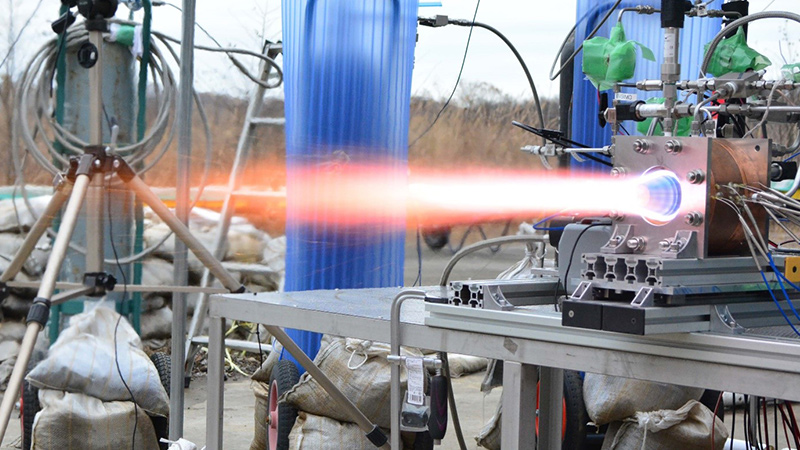
\includegraphics[width=\textwidth]{../figs/rde.jpg}
\caption{Nagoya University 900 N Rotating Detonation Engine \cite{nagoya}}
\end{figure}
\end{columns}
\end{frame}

\begin{frame}{Objectives}
\begin{itemize}
\item Implement and test AMR techniques for simulations of detonations found within RDEs and PDEs within OpenFOAM \cite{weller}, which has:
\begin{itemize}
\item geometric flexibility 
\item consistent input structure (easy to transition between solvers)
\item good documentation
\item open source, GNU GPL
\end{itemize}
\item Build a framework on previous work by Towery \cite{towery1} and TESLa at CU Boulder for further RDE and PDE research 
\end{itemize}
\end{frame}

\begin{frame}{Previous Work}
\begin{itemize}
\item Towery \textit{et. al.} \cite{towery1} examined PDEs and RDEs with static grids with inviscid Euler equations using an in-house Fortran parallelized code, also focusing on turbulence modeling 
\item Marcantoni \textit{et. al.} \cite{marcantoni} developed \texttt{rhoReactingRfFoam}, a non-AMR OpenFOAM solver for detonations 
\item Berger and Jameson \cite{berger1985} used and developed adaptive mesh refinement routines to solve the Euler equations 
\item Deiterding \cite{deiterding} used the Berger and Colella \cite{berger1989} AMR routines to simulate detonations with the Euler equations, developing and implementing parallelization and distributed computing 
\end{itemize}
\end{frame}

\begin{frame}{Previous Work (ii)}
\begin{itemize}
\item Yi \textit{et. al.} \cite{yi} explored numerical simulations of RDEs in three dimensions, exploring overall flow-field and comparing to one- and two-dimensional simulations 
\item Schwer and Kailasanath \cite{schwer1} examined effects of different hydrocarbon fuels in RDEs as well as numerical methods for simulating them 
\item Li \textit{et. al.} \cite{li} used the Berger-Oliger AMR routines \cite{berger1984} and simulated detonations, noting the presence of cellular detonation structure 
\item Kim and Kim \cite{kim} simulated confined detonations in OpenFOAM with seven-step chemistry and compared to experimental results 
\end{itemize}
\end{frame}

